
\chapter{Proposed Systems}
\justify

This chapter provides a detailed overview of the \textbf{{\myprojectname}}. It outlines the project's main aim of collecting information for law enforcement purposes, along with the objectives, scope, assumptions, dependencies, and system requirements essential for its implementation.

\section{Objectives}
The primary objective of the \textbf{{\myprojectname}} is to provide law enforcement agencies with a rapid and efficient means of analyzing call data records (CDRs) and tower dump data. By harnessing the power of C-Trace's sophisticated features and tools, investigators can swiftly identify suspects and establish connections, even in cases where other investigative leads may be limited or scarce. C-Trace acts as a force multiplier, empowering investigators to make informed decisions and progress their investigations more effectively.Specifically, the objectives are as follows:
\begin{enumerate}[label=\arabic*.]
    \item To collect various types of information from individuals, including:
    \begin{itemize}
        \item Vehicle details
        \item Location data
        \item IMEI numbers
        \item Phone numbers
        \item PAN numbers
        \item MNP details
        \item IP information and more
    \end{itemize}
    \item To develop a caller ID app named "Call One" that collects users' contacts, call logs, emails, and location information.
    \item To store the collected data securely in a PostgreSQL database for law enforcement agencies to access.
    \item To implement data validation and verification processes to ensure the accuracy and reliability of collected information.
    \item To integrate advanced analytics and data mining techniques to extract valuable insights from the collected data, aiding law enforcement in investigations and intelligence gathering.
\end{enumerate}

\section{Scope}
The scope of the "{\myprojectname}" app includes the following key components:
\begin{enumerate}[label=\arabic*.]
    \item \textbf{Collection of People Information}: Scraping various information from websites and mobile apps such as social media sites and e-commerce wesites.
    \item \textbf{Collection of Users' Contacts and Call Logs}: The app will extract contact information from various sources, including websites and apps, through web scraping techniques. Call logs will be retrieved from users' devices to track incoming and outgoing calls.
    \item \textbf{Collection of Emails}: The app will access users' email accounts to gather relevant email data.
    \item \textbf{Collection of Location Information}: Location data will be obtained to track the geographical whereabouts of users.
    \item \textbf{Data Storage}: All collected data will be securely stored in a database accessible to law enforcement agencies for analysis and investigations.
    \item \textbf{Real-time Data Updates}: Implementing mechanisms to ensure that the collected data is continuously updated in the database, reflecting the latest information available.
    \item \textbf{Data Aggregation}: Aggregating data from multiple sources to provide a comprehensive overview for law enforcement agencies, facilitating efficient decision-making.
    \item \textbf{Data Visualization}: Incorporating data visualization tools and dashboards to present information in a visually appealing and understandable format, aiding in data analysis and interpretation.
    \item \textbf{Scalability}: Designing the system to be scalable, allowing for future enhancements and additions to accommodate evolving data collection requirements.
\end{enumerate}

\section{Assumptions}
The successful implementation of the \textbf{{\myprojectname}} is based on the following assumptions:
\begin{enumerate}[label=\arabic*.]
    \item \textbf{Availability of Necessary APIs}: The app assumes access to APIs or scraping techniques to collect data from various sources.
    \item \textbf{User Consent}: Users are assumed to provide consent for the collection of their data as per legal and ethical standards, with provisions for law enforcement access.
    \item \textbf{Data Security Measures}: Adequate security measures will be implemented to protect the collected data, especially sensitive information, from unauthorized access or breaches.
    \item \textbf{Data Retention Policies}: Adhering to data retention policies to ensure that collected information is stored for an appropriate duration, considering legal and operational requirements.
    \item \textbf{Continuous Monitoring}: Implementing continuous monitoring mechanisms to detect and respond to any unauthorized access attempts or security breaches promptly.
\end{enumerate}

\section{Dependencies}
The proposed system is dependent on the following factors for its successful implementation:
\begin{enumerate}[label=\arabic*.]
    \item \textbf{Technical Infrastructure}: Availability of necessary hardware, software, and network infrastructure to support app functionality.
    \item \textbf{Legal Compliance}: Adherence to legal regulations and privacy policies governing data collection and usage, including provisions for law enforcement access.
    \item \textbf{User Adoption}: User acceptance and adoption of the "Call One" app, with awareness of its law enforcement data collection purpose.
    \item \textbf{Interoperability}: Ensuring interoperability with existing systems and databases used by law enforcement agencies to facilitate seamless data sharing and integration.
    \item \textbf{Training and Support}: Providing training sessions and ongoing support to law enforcement personnel using the system, ensuring effective utilization and maximizing its benefits.
\end{enumerate}

\section{System Requirements}

The system requirements for implementing the {\myprojectname} include:

\begin{figure}
    \centering
    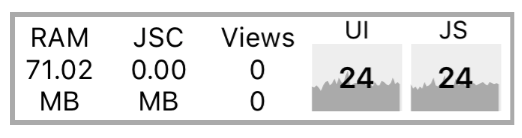
\includegraphics[width=0.90\linewidth]{Media//minreq.png}
    \caption{Minimum requirements for react native app}
    \label{fig:Minimum requirements for react native app}
\end{figure}

\begin{enumerate}[label=\arabic*.]
    \item \textbf{Compatible System}:  .NET Framework app on Windows, Generally need a compatible Windows OS (like Windows 7, 8, 8.1, or 10) and the specific version of you.NET Framework required by the app installed on your system.
    \item \textbf{Compatible Devices}: The Call One app should be compatible with a range of devices, including smartphones and tablets.
    \item \textbf{Data Collection Modules}: Modules for collecting contacts, call logs, emails, and location information.
    \item \textbf{Database Management System}: A robust database management system for secure data storage and retrieval, with provisions for law enforcement access.
    \item \textbf{Security Features}: Encryption mechanisms, access controls, and authentication protocols to ensure data security, particularly for law enforcement-related data.
    \item \textbf{User Interface}: Intuitive user interface design for easy navigation and interaction with app features, including law enforcement functionalities.
    \item \textbf{Audit Trails}: Incorporating audit trail functionality to track and record all access and modifications to the data, maintaining transparency and accountability.
    \item \textbf{Compliance Checks}: Implementing automated compliance checks to ensure that data collection and storage practices align with regulatory requirements and standards.
    \item \textbf{Regular Updates and Maintenance}: Committing to regular updates and maintenance of the app and database system to address security vulnerabilities and improve overall performance.
    \item \textbf{Performance Monitoring}: Deploying performance monitoring tools to assess system performance, identify bottlenecks, and optimize resource utilization for optimal user experience.
    \item \textbf{Feedback Mechanisms}: Integrating feedback mechanisms within the app for users and law enforcement agencies to provide input, suggestions, and report any issues or concerns regarding data collection and usage.
\end{enumerate}
